% =====================================================================
% Documentación técnica formal — Proyecto Capstone "Evento Cultural"
% Compilación: pdflatex -interaction=nonstopmode main.tex  (dos pasadas)
% =====================================================================
\documentclass[11pt,a4paper]{article}

\usepackage[utf8]{inputenc}
\usepackage[T1]{fontenc}
\usepackage[spanish]{babel}
\usepackage{lmodern}
\usepackage[margin=2.4cm]{geometry}
\usepackage{graphicx}
\usepackage{float}
\usepackage{xcolor}
\usepackage{booktabs}
\usepackage{longtable}
\usepackage{array}
\usepackage{enumitem}
\usepackage{caption}
\setlength{\emergencystretch}{3em}
\sloppy

\definecolor{terracota}{HTML}{C9622D}
\definecolor{verdes}{HTML}{1F5C57}
\definecolor{rojo}{HTML}{B03A3A}
\definecolor{azulurl}{HTML}{1F4E79}
\usepackage[colorlinks=true,linkcolor=azulurl,urlcolor=azulurl]{hyperref}

\graphicspath{{Diagramas/}}
\captionsetup{font=small,labelfont=bf}
\renewcommand{\tablename}{Tabla}

\newcommand{\pendiente}{\textcolor{rojo}{\textbf{Pendiente de completar por el equipo.}}}
\newcommand{\seccionpendiente}[1]{\textcolor{rojo}{\textbf{Pendiente de completar por el equipo:} #1}}

\title{}
\author{}
\date{}

\begin{document}

% ---------------------------------------------------------- PORTADA
\begin{titlepage}
\centering
{\color{terracota}\rule{\textwidth}{2pt}}\\[0.6cm]
{\Large \textsc{Duoc UC -- Sede Maipú}}\\[0.2cm]
{\large Capstone 2026 -- Asignatura APT122}\\[1.4cm]
{\color{terracota}\Huge \textbf{Evento Cultural}}\\[0.5cm]
{\LARGE Documentación Técnica del Proyecto}\\[0.4cm]
{\large Plataforma chilena de eventos culturales}\\[1.2cm]
{\color{terracota}\rule{\textwidth}{1pt}}\\[1.2cm]

\begin{minipage}{0.82\textwidth}
\renewcommand{\arraystretch}{1.35}
\begin{center}
\begin{tabular}{>{\bfseries}l l}
Integrante & Rol principal \\ \midrule
Roberto Riffo & Líder de proyecto / Frontend / UX \\
José Miguel Moncada & Base de datos / QA \\
David Herrera & Backend e integraciones \\
\end{tabular}
\end{center}
\vspace{0.2cm}
{\small Roles según el design brief aprobado en Fase 1 (\textit{design\_brief\_capstone.docx}).}
\end{minipage}

\vspace{1.2cm}
\begin{minipage}{0.82\textwidth}
\small
\textbf{Stack del sistema:} Python (scraper con conectores, NVIDIA NIM y checkpoints SQLite),
Supabase/PostgreSQL con Row Level Security, Edge Functions (registro, cuenta, publicación, moderación y recuperación),
Angular 22 + Ionic 9 (web y móvil, catálogo real y autenticación directa vía \texttt{@supabase/supabase-js}),
Leaflet + OpenStreetMap (mapa interactivo con pines georreferenciados) y GitHub Actions para automatización.
\end{minipage}

\vfill
{\large Versión 1.3}\\[0.2cm]
{\large 31 de octubre de 2026}\\[0.4cm]
{\small Revisión de cierre (Fase 3): agrega estándares de desarrollo, estructura de evidencias y referencias.\\
Revisión contrastada con el código local actual; resultados históricos separados\\
de las verificaciones de cierre pendientes. Ver Respuesta\_Rubrica\_Fase2.md.\\
Las omisiones se declaran como \textcolor{rojo}{\textbf{pendientes del equipo}} dentro
de este mismo documento.}\\[0.3cm]
{\color{terracota}\rule{\textwidth}{2pt}}
\end{titlepage}

% ---------------------------------------------------------- ÍNDICE
\tableofcontents
\newpage

% ---------------------------------------------------------- INTRODUCCIÓN
\section{Introducción y alcance}
\label{sec:intro}

Este documento consolida el estado técnico de Evento Cultural al 31-10-2026 a partir
del código local actual, las funciones Edge y configuración de la aplicación. Conserva
como línea base los requerimientos de Fase 1, el modelo de datos y la evidencia del
scraper y QA de Fase 2. No certifica el esquema remoto ni reemplaza una ejecución de pruebas.

\textbf{Convención de honestidad documental:} este documento distingue explícitamente entre
lo \emph{implementado} (respaldado por código), lo \emph{parcial} (respaldado solo en parte)
y lo \emph{pendiente} (información humana o trabajo futuro). Nada se afirma como terminado
sin respaldo; los puntos abiertos se marcan con \pendiente

\subsection{Estructura del sistema}

El sistema se compone de tres bloques independientes que se comunican a través de la base
de datos: el \textbf{scraper} (recolección y enriquecimiento de datos), la \textbf{base de
datos} (catálogo canónico en Supabase/PostgreSQL) y el \textbf{frontend} (aplicación web y
móvil), con \textbf{GitHub Actions} como automatización de la ejecución del scraper
(ver Figura~\ref{fig:arq} en la Sección~\ref{sec:arq}).

\subsection{Respuesta a la evaluación anterior}
La planilla de Fase 2 registra 74/100 y nota 5,1. Los descuentos están en los indicadores
3 (15/25), 4 (3/5), 5 (3/5), 6 (12/20) y 8 (6/10). No contiene observaciones narrativas
específicas. Se corrigen precisión técnica, estado del producto, fuentes y trazabilidad;
la entrega en Git y el dominio oral del equipo requieren evidencia adicional.
El registro \texttt{Respuesta\_Rubrica\_Fase2.md} vincula cada indicador con acciones
sin prometer una nueva calificación. Código implementado no equivale a prueba aprobada.

% Revisión documental de Fase 3: 31-10-2026.
\section{Arquitectura general del sistema}
\label{sec:arq}
\subsection{Alcance y fuente de verdad}
Esta revisión toma como fuente principal el código local de
\nolinkurl{EventoCultural_Integrado/EventoCultural_Integrado}. La rama de referencia
es \url{https://github.com/sunsitox/Proyecto_Capston_Evento_Cultural/tree/deploy/vercel-preview}.
No se certifica igualdad entre la copia local y esa rama ni que todas las funciones
locales estén desplegadas. Se distingue implementación, configuración remota y
verificación de extremo a extremo.

\begin{itemize}[leftmargin=1.4em]
\item \textbf{Recolección:} scraper Python independiente, con conectores, saneamiento,
NVIDIA NIM selectivo y checkpoints SQLite. Su evidencia operativa conservada corresponde
al ciclo del 11-10-2026; no constituye una nueva ejecución del scraper.
\item \textbf{Persistencia:} Supabase/PostgreSQL, catálogo y perfiles con políticas RLS;
Supabase Auth para sesiones y Storage para avatares.
\item \textbf{Cliente:} SPA Angular 22 e Ionic 9, con servicios TypeScript y signals.
Consulta catálogo y autenticación mediante \texttt{@supabase/supabase-js}.
El código Python de \texttt{backend/} es legado y no es una dependencia del flujo web actual.
\item \textbf{Servidor:} Supabase Edge Functions para operaciones privilegiadas:
\texttt{registrar-cuenta}, \texttt{admin-account}, \texttt{publicar-evento},
\texttt{admin-eventos}, \texttt{reset-password-request},
\texttt{reset-password-confirm} y \texttt{recomendaciones-semanal}.
La clave de servicio pertenece exclusivamente al servidor.
\item \textbf{Entrega:} Vercel para la SPA, GitHub Actions para el scraper y Capacitor
para Android. No se utiliza Docker en la estrategia adoptada.
\end{itemize}

\begin{figure}[H]\centering
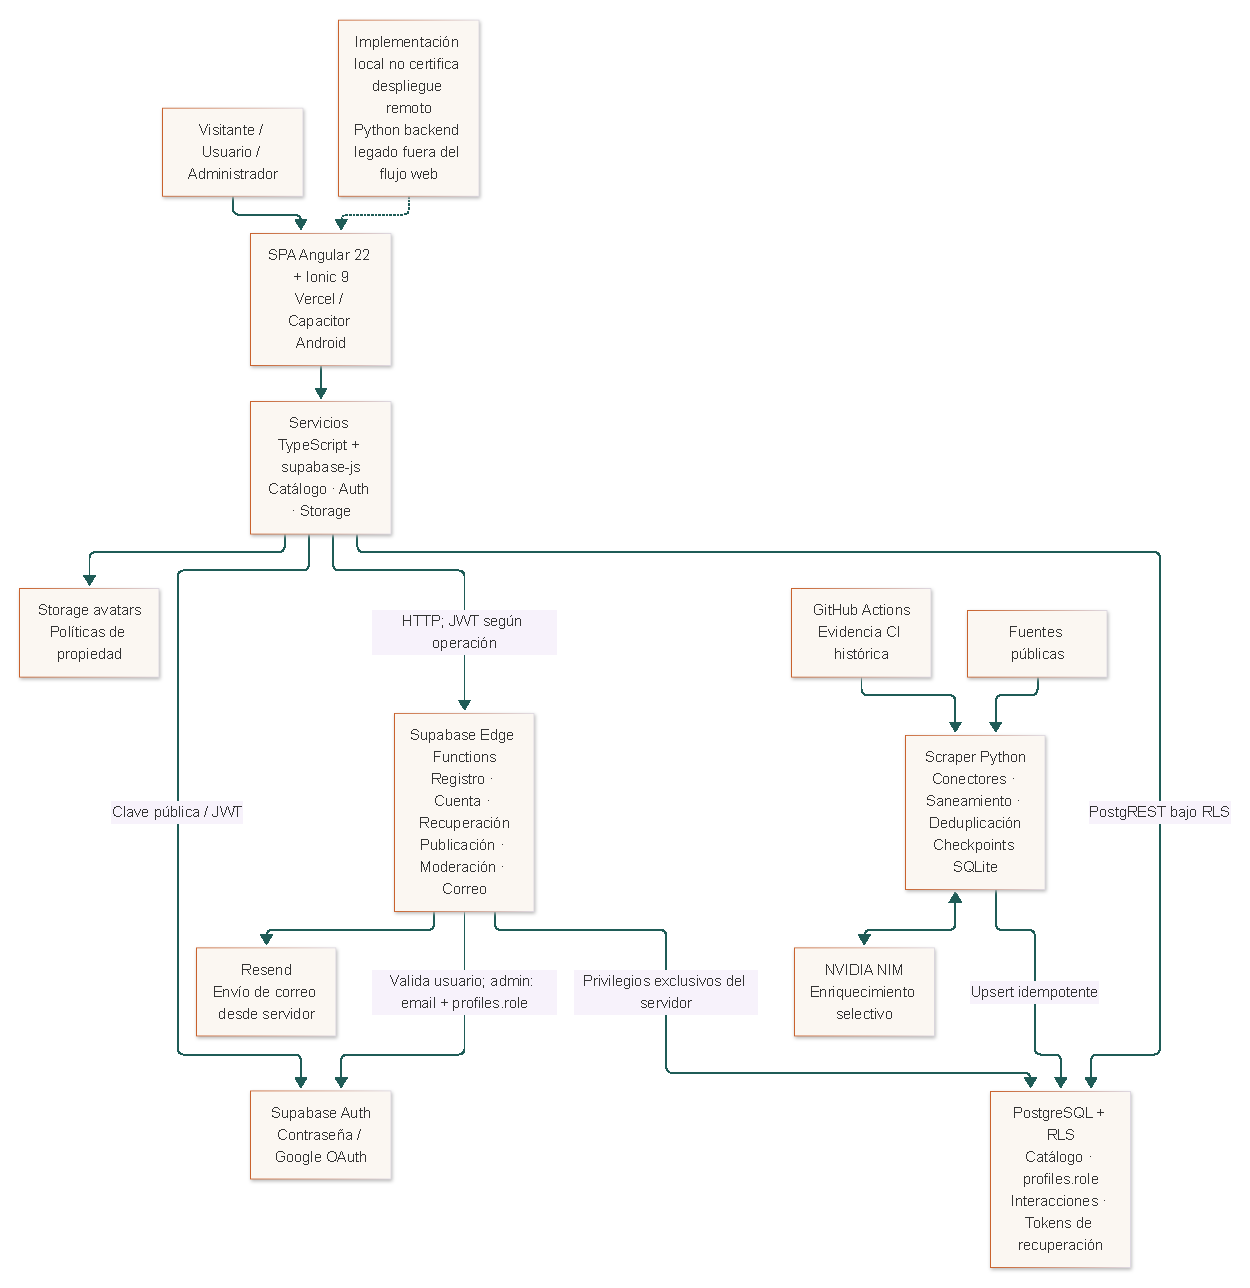
\includegraphics[width=\textwidth,height=0.70\textheight,keepaspectratio]{01_arquitectura_general.pdf}
\caption{Arquitectura actual; fuente editable: Diagramas/01\_arquitectura\_general.mmd.}
\label{fig:arq}\end{figure}

\subsection{Contratos y límites de confianza}
\begin{longtable}{p{3.1cm}p{4.0cm}p{7.0cm}}
\toprule Origen y destino & Contrato & Regla de acceso \\\midrule\endhead
Cliente a Supabase & Catálogo mediante PostgREST; sesión mediante Auth & Clave pública y JWT del usuario; las políticas RLS gobiernan los datos. \\
Registro a función Edge & Correo, contraseña y nombre & Crea cuenta confirmada mediante Admin API; luego el cliente inicia sesión. No comprueba la propiedad del buzón. \\
Usuario a publicar-evento & Datos validados del evento y JWT & Identidad obtenida con getUser; crea evento draft y no acepta status/source\_id del cliente. \\
Administrador a admin-eventos & Listado y acciones de moderación & Valida JWT, proveedor email y profiles.role=admin antes de utilizar privilegios de servicio. \\
Recuperación a funciones Edge & Solicitud por correo y confirmación con token & JWT firmado y registro password\_reset\_tokens con caducidad y marca de uso; requiere migración y secretos. \\
Servidor a correo & API de Resend & Clave privada en el entorno de funciones. Envío implementado no equivale a recepción demostrada. \\
\bottomrule\end{longtable}

\section{Arquitectura del scraper}
\label{sec:scraper}
El pipeline carga fuentes declarativas, selecciona conectores por Strategy/Factory,
sanea y deduplica eventos, normaliza ubicaciones, exporta JSON/CSV y sincroniza
Supabase por upsert. Los checkpoints SQLite permiten reanudar trabajo y reutilizar
resultados de IA de eventos sin cambios. El límite configurado de NVIDIA es 40 RPM;
no se presenta como una garantía contractual del proveedor.

\begin{figure}[H]\centering
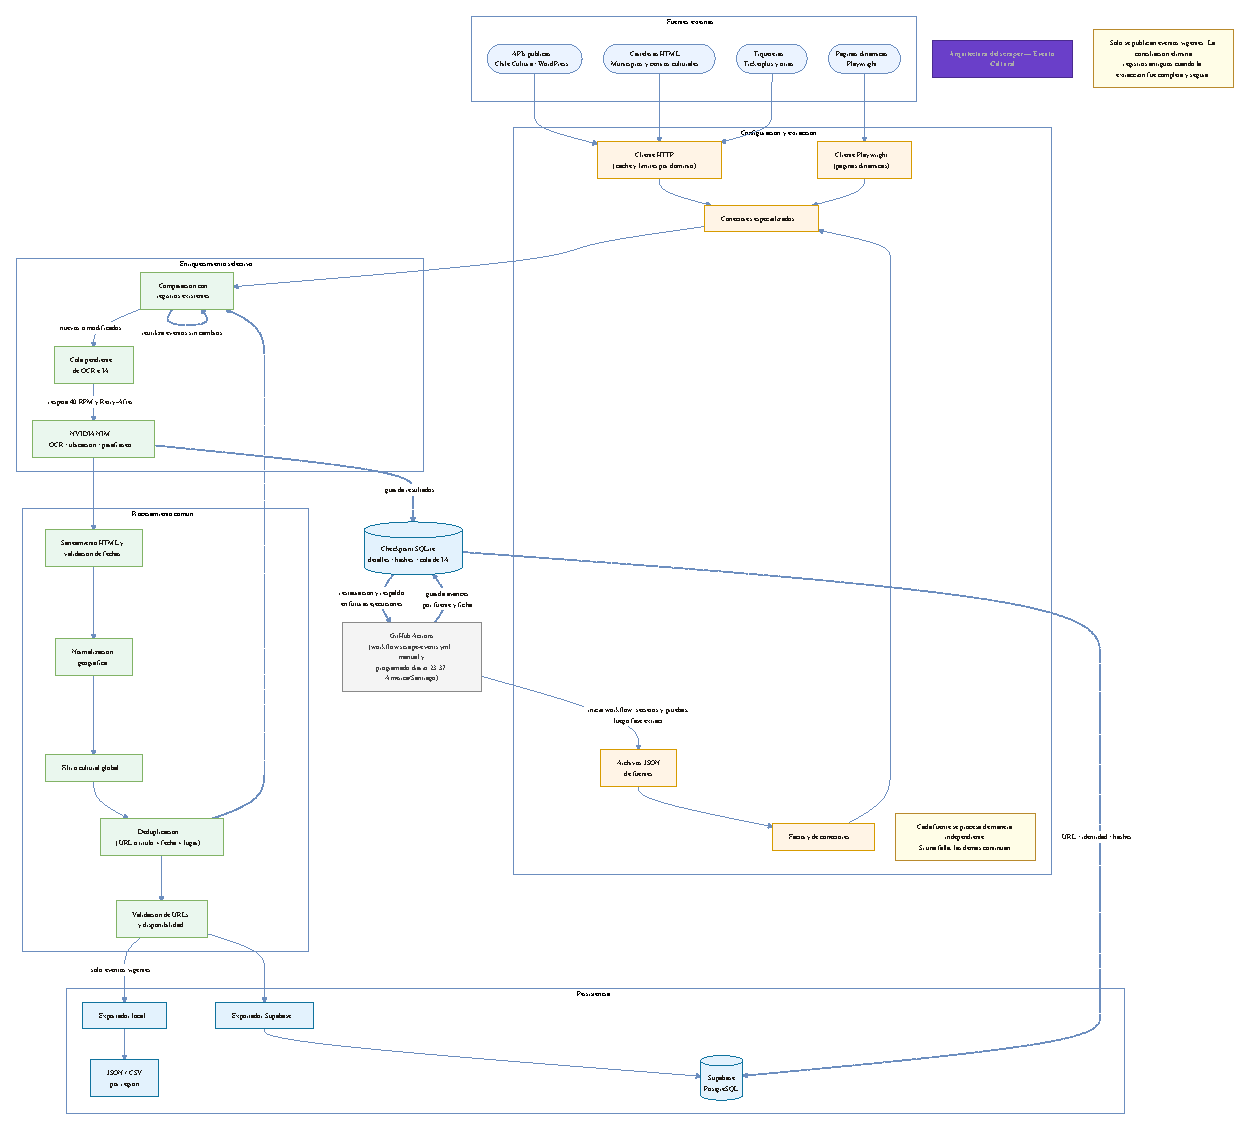
\includegraphics[width=0.94\textwidth]{07_arquitectura_scraper.pdf}
\caption{Pipeline del scraper conservado de la línea base; verificar su inventario vigente antes del cierre.}
\label{fig:scraper-arq}\end{figure}

El inventario de 21 fuentes permanentes y una estacional y las ejecuciones de CI
corresponden a evidencia histórica. No se infiere que todas sigan disponibles hoy.
Los conectores aíslan fallos por fuente; la conciliación y el borrado de vencidos
dependen de la configuración y de una extracción completa. GitHub Actions no garantiza
puntualidad: el desfase del run 25 sigue registrado como DEF-CI-001.

\section{Arquitectura del frontend}
\label{sec:frontend}
\subsection{Stack y organización}
Según \texttt{package.json}: Angular 22.0.1, Ionic 9, TypeScript 6,
Capacitor 8, supabase-js 2, Leaflet 1.9.4, RxJS 7.8 y Vitest 4 con jsdom.
\texttt{core/} concentra modelos y servicios; \texttt{pages/} las pantallas;
\texttt{features/home/} los layouts; y \texttt{layout/} la navegación adaptativa.
Las versiones resueltas deben reproducirse con \texttt{package-lock.json}.

\begin{figure}[H]\centering
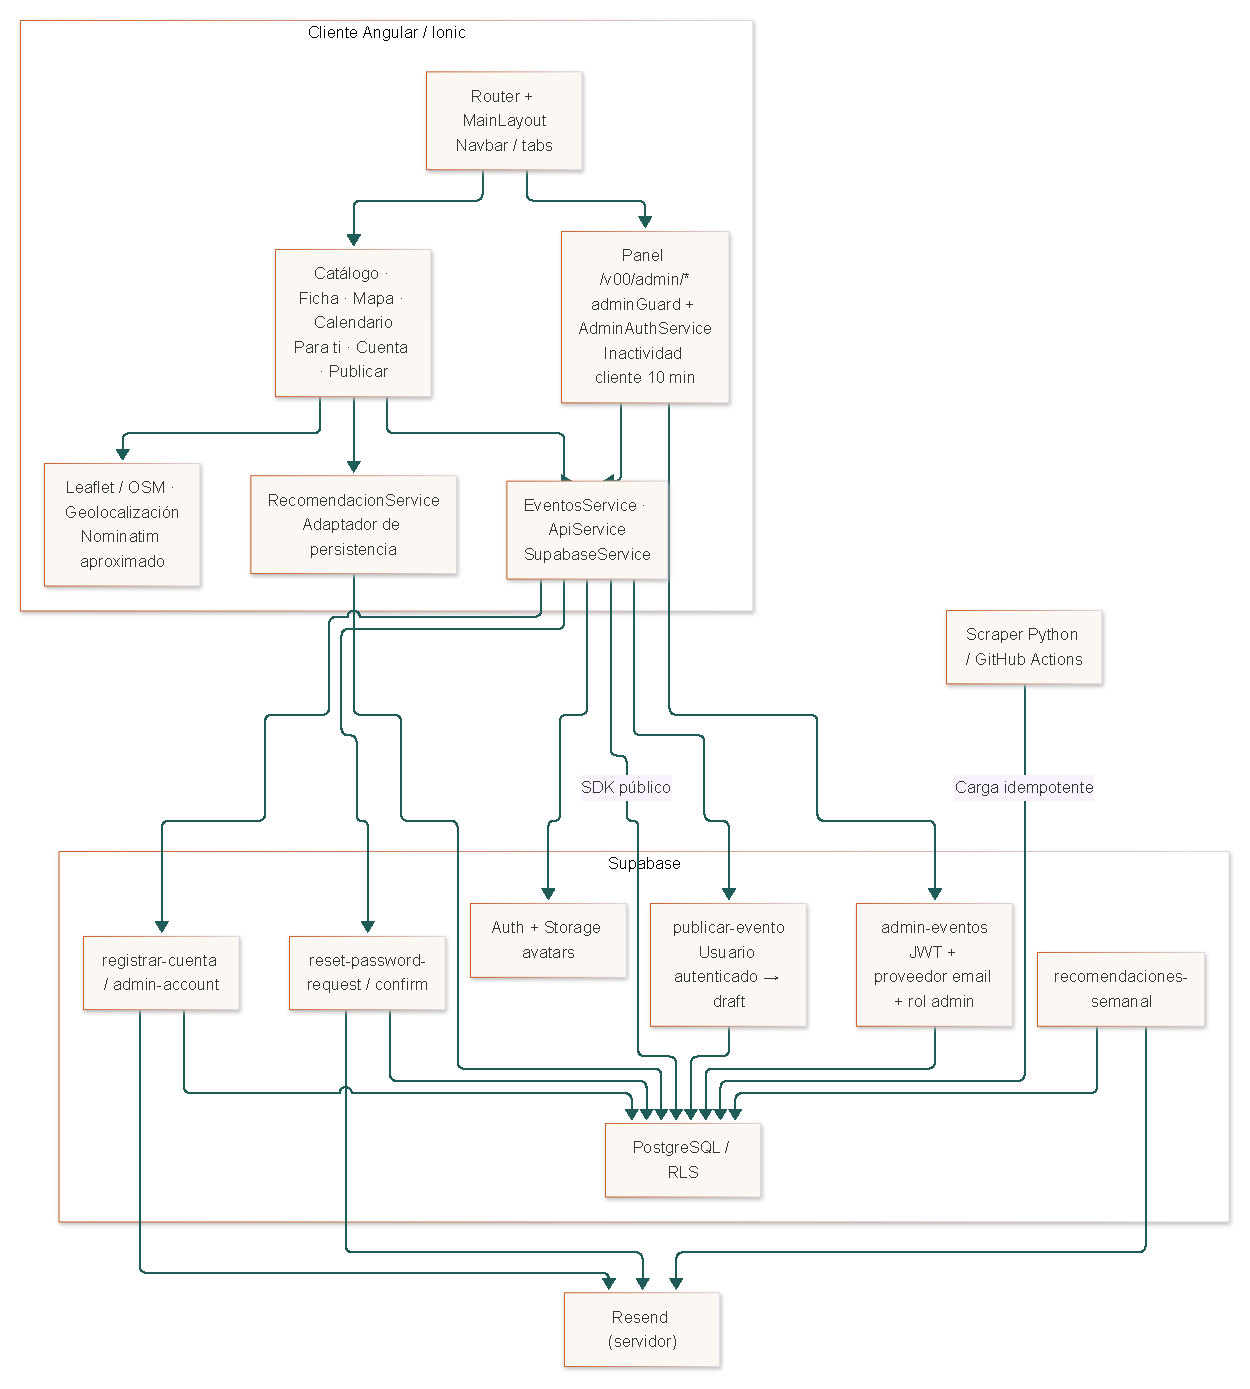
\includegraphics[width=0.95\textwidth,height=0.68\textheight,keepaspectratio]{02_componentes.pdf}
\caption{Componentes actuales y separación cliente/servidor.}
\label{fig:comp}\end{figure}

\subsection{Descubrimiento y personalización}
El catálogo publicado alimenta búsqueda, filtros combinados, detalle, calendario y
mapa Leaflet/OpenStreetMap. Nominatim aporta geocodificación de respaldo con cola,
caché y límites; los resultados aproximados no sustituyen coordenadas verificadas.
La geolocalización usa Capacitor en Android y alternativa web.
Las recomendaciones se calculan por señales de interés, no por un modelo generativo:
\texttt{RecomendacionService} calcula afinidad y razones; el adaptador de persistencia
almacena interacciones en \texttt{user\_event\_interactions} y preferencias en metadata.
Los invitados mantienen estado en memoria. El respaldo de eventos de demostración no
debe confundirse con una consulta remota exitosa.

\subsection{Cuenta y perfil}
El registro principal llama \texttt{registrar-cuenta}, que crea el usuario con
\texttt{email\_confirm=true}; el cliente ejecuta \texttt{signInWithPassword} sin
exigir verificación del buzón. La función intenta enviar un correo de registro exitoso
por Resend. Existe respaldo legacy con \texttt{signUp}: si la función no está disponible,
puede reaparecer la confirmación de Supabase. Por tanto, la experiencia solicitada
requiere desplegar y configurar la función, no solo cambiar el formulario.

El perfil permite editar nombre, contraseña e imagen. Storage utiliza el bucket
\texttt{avatars}; el metadata \texttt{avatar\_url\_custom} tiene prioridad sobre la imagen
OAuth, y esta se utiliza si no hay imagen propia. La identidad reactiva alimenta perfil
y navegación. Google OAuth tiene botón y callback implementados; su configuración remota
y la recepción de correos no se certifican por inspección de código.
La recuperación actual usa las funciones \texttt{reset-password-request/confirm} y
\texttt{/restablecer-contrasena?token=...}, no únicamente el flujo antiguo de GoTrue.

\subsection{Administración y publicación}
Las rutas \texttt{/v00/admin/*} requieren \texttt{adminGuard}; no enlazarlas públicamente
no constituye una medida de autorización. \texttt{AdminAuthService} consulta
\texttt{profiles.role} y solo admite \texttt{admin}, con proveedor email: visitor,
editor y Google son rechazados. El rol editable de metadata no es autoridad administrativa.
La función \texttt{admin-eventos} repite las comprobaciones en el servidor.
El cliente cierra la sesión tras 10 minutos sin interacción, comprobados cada 15 segundos,
y redirige al ingreso con aviso. La última actividad se reinicia al recargar; no es un
timeout absoluto persistido ni una revocación impuesta por el servidor.

La publicación autenticada crea un borrador mediante \texttt{publicar-evento};
\texttt{admin-eventos} implementa listado administrativo, publicación y supresión.
El dashboard calcula métricas del catálogo cargado en el cliente: no equivale a analítica
comercial ni a estadísticas certificadas de uso. La ocultación de fuentes en el navegador
no equivale a detener el scraper ni a persistir una decisión global.

\subsection{Despliegue y pendientes}
\texttt{angular.json} genera \texttt{www}; \texttt{vercel.json} ya incluye la reescritura
SPA a \texttt{/index.html}. Existe proyecto Android y APK debug local; esto no demuestra
instalación, GPS u OAuth en dispositivo físico ni publicación en tienda.
Quedan por registrar: regresión del ciclo QA histórico, pruebas remotas de autorización,
correo y recuperación, aislamiento entre usuarios, pruebas nativas y mediciones de
rendimiento/accesibilidad. Ninguno de esos resultados se deduce de una compilación.

% =====================================================================
% PARTE 2 — Modelo de datos y diagramas UML
% =====================================================================

\section{Modelo de datos (Supabase / PostgreSQL)}
\label{sec:datos}

\subsection{Fuente del modelo}
\textbf{Corte de Fase 3 (31-10-2026):} el ER representa la línea base del catálogo,
no un volcado del esquema remoto actual. El código incorpora perfiles para autorización,
interacciones para recomendaciones, Storage de avatares y la migración local
\nolinkurl{20261024000100_password_reset_tokens.sql}. La tabla de tokens de recuperación
almacena identificador, usuario, correo, vencimiento y marca de uso; su despliegue se debe
verificar antes de probar recuperación. Auth referencia realmente \texttt{auth.users};
el nombre \texttt{auth\_users} del dibujo es una representación conceptual.


El modelo se documenta a partir de la documentación de base de datos incluida en el
entregable del scraper de Fase 2, el DBML editable, el diccionario de tablas
(DOCX, versión documentada al 03-10-2026) y el diagrama ER de Fase 1
(\texttt{DB\_evento\_cultural.pdf}). Las migraciones SQL no se incluyeron en la copia local
entregada, pero están disponibles en el repositorio oficial del proyecto
(\url{https://github.com/sunsitox/sunsitox-Scraper_de_eventos_culturales}).

\begin{figure}[H]
\centering
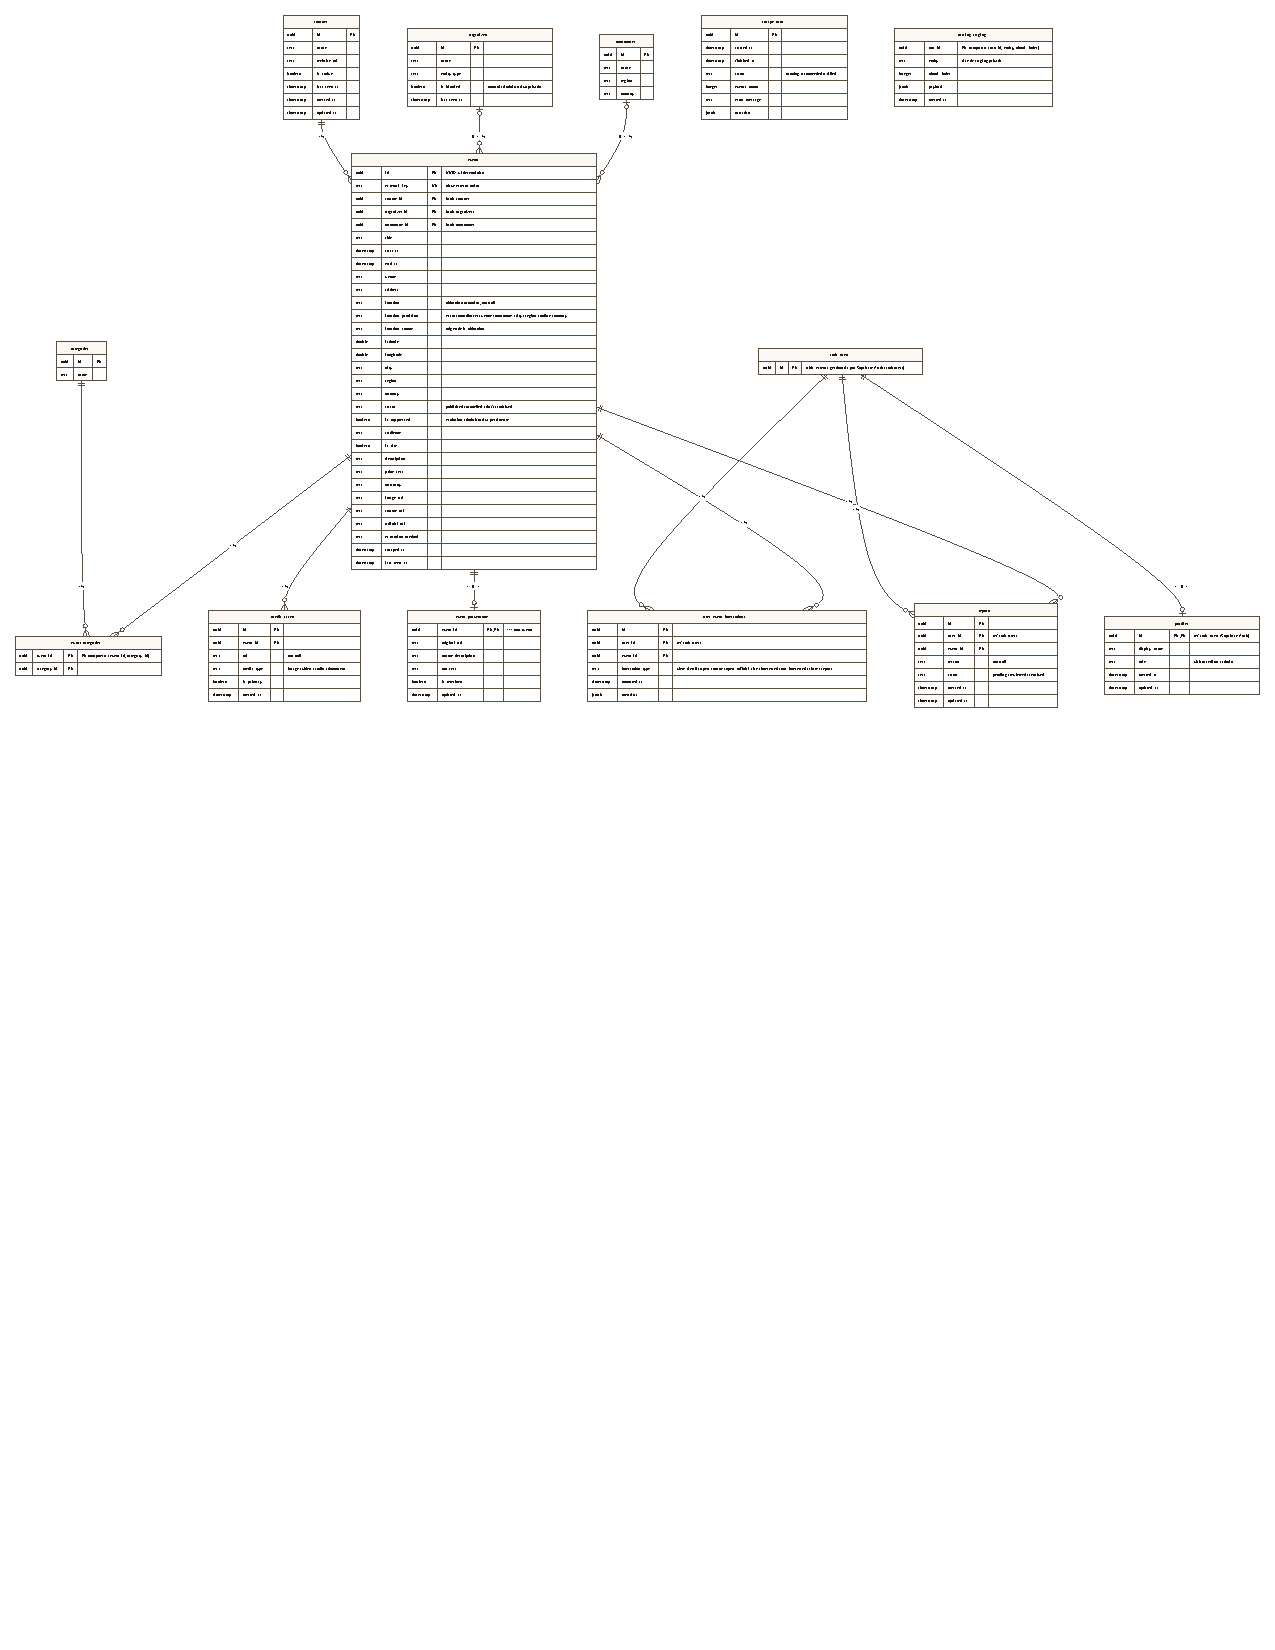
\includegraphics[width=0.95\textwidth]{06_modelo_er.pdf}
\caption{Modelo entidad--relación (fuente editable: \texttt{Diagramas/06\_modelo\_er.mmd}, Mermaid).}
\label{fig:er}
\end{figure}

\subsection{Tablas y finalidad}

\begin{table}[ht]
\centering\small
\renewcommand{\arraystretch}{1.25}
\begin{tabular}{l p{4.1cm} p{6.6cm}}
\toprule
\textbf{Grupo} & \textbf{Tabla} & \textbf{Finalidad} \\
\midrule
Ingesta y catálogo & \texttt{sources} & Agenda, municipalidad, ticketera o sitio de origen \\
 & \texttt{organizers} & Institución responsable del evento \\
 & \texttt{communes} & Ubicación administrativa normalizada \\
 & \texttt{categories} & Etiquetas temáticas, de formato o audiencia \\
 & \texttt{events} & Registro canónico del evento consolidado (37 columnas) \\
 & \texttt{event\_categories} & Relación N:M entre eventos y categorías \\
 & \texttt{media\_assets} & Imágenes y futuros multimedia \\
 & \texttt{scrape\_runs} & Bitácora de ejecuciones locales y de GitHub Actions \\
 & \texttt{event\_provenance} & Evidencia privada: URL original, descripción de la fuente, texto OCR y marca de reescritura \\\
Aplicación & \texttt{profiles}, \nolinkurl{user_event_interactions}, \texttt{reports} & Perfiles e interacciones usados por la aplicación; reports no se declara como flujo completo; \texttt{profiles} referencia a \texttt{auth\_users}, la tabla externa de Supabase Auth \\
Staging & \texttt{catalog\_staging} & Área privada de carga por lotes (payload JSON) antes de publicar el catálogo \\
\bottomrule
\end{tabular}
\caption{Tablas del modelo de datos según el diccionario y el DBML del proyecto.}
\label{tab:tablas}
\end{table}

Los identificadores de eventos, organizadores, comunas y categorías son \textbf{UUID v5
deterministas} derivados de claves externas: ejecutar dos veces el mismo scraping actualiza
las filas (upsert) sin crear duplicados. El campo \texttt{categories} se normaliza en
\texttt{categories} y \texttt{event\_categories}, conservando la relación muchos-a-muchos.

\subsection{Seguridad (Row Level Security) y ciclo de carga}

La migración de RLS habilita Row Level Security en todas las tablas; \texttt{scrape\_runs}
no tiene lectura pública; el usuario no puede cambiar su propio rol ni el estado de sus
reportes desde el frontend; la vista \texttt{public\_event\_catalog} hereda las reglas RLS y
no expone eventos suprimidos ni organizadores bloqueados.

En el ciclo de carga, la sincronización identifica coincidencias por URL o clave compuesta,
carga por lotes (\texttt{SUPABASE\_BATCH\_SIZE}) y registra cada ejecución en
\texttt{scrape\_runs} como \texttt{running}, \texttt{succeeded} o \texttt{failed}. La
repetición idempotente es el mecanismo de recuperación ante cargas parciales.

\subsection{Limitaciones declaradas}

Sin marca explícita de eventos de día completo; \texttt{price\_text} no permite comparación
numérica; categorías sin jerarquía almacenada; registros de Chile Cultura que pueden ser
directorios y no eventos fechados; etiqueta inválida conocida (\texttt{Calendar\_Month
Inscribirse}); borrado físico de vencidos solo con
\texttt{SUPABASE\_DELETE\_EXPIRED=true}.

\section{Diagramas UML}
\label{sec:uml}

Los cuatro diagramas UML exigidos por el anexo metodológico se escriben como código fuente
Mermaid (\texttt{.mmd}) y se renderizan a PDF con \texttt{mermaid-cli}, en la carpeta
\texttt{Diagramas/} de esta misma sección. Los casos de uso se derivan de la matriz MoSCoW de
Fase 1 y de las páginas realmente implementadas en el frontend. Todos los diagramas (01--07)
comparten un estándar visual único (paleta institucional, tipografía Arial, flechas
reforzadas), declarado dentro de cada archivo \texttt{.mmd}, y fueron regenerados el
27-09-2026 al migrar de Draw.io a Mermaid para automatizar el trazado de líneas y facilitar
el mantenimiento; el diagrama entidad--relación (06) fue corregido y reexportado el
03-10-2026 para alinearlo con el diccionario de tablas y el DBML vigentes; los
diagramas 01 (arquitectura general), 02 (componentes) y 04 (secuencia) fueron
regenerados el 10-10-2026 para reflejar la integración del sistema: la API
intermedia (\texttt{supabase\_backend.py}) entre el frontend y Supabase, la
autenticación real con regreso OAuth en \texttt{/auth/callback} y el mapa interactivo. En esta revisión los diagramas 01, 02 y 04 sustituyen la API Python histórica por SDK directo y funciones Edge.

\subsection{Casos de uso}

\begin{figure}[H]
\centering
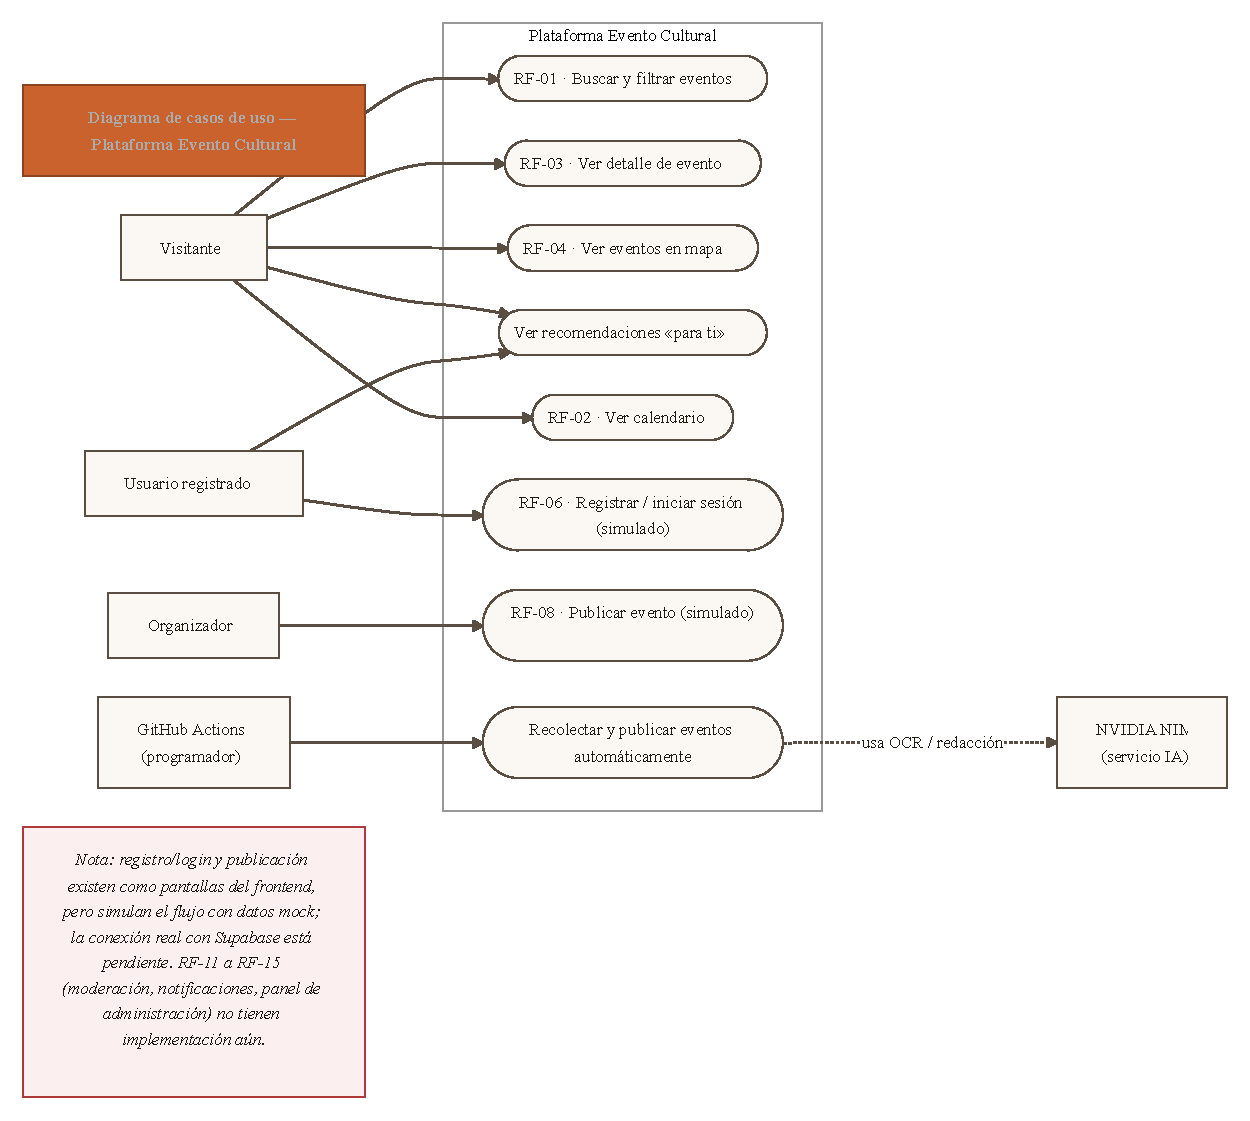
\includegraphics[width=0.9\textwidth]{03_casos_de_uso.pdf}
\caption{Casos de uso de la plataforma (fuente editable: \texttt{Diagramas/03\_casos\_de\_uso.mmd}, Mermaid).}
\label{fig:uc}
\end{figure}

El visitante consulta catálogo, mapa y calendario; la cuenta autenticada gestiona su perfil, recibe recomendaciones y envía borradores mediante publicar-evento. El administrador de proveedor email y rol admin modera mediante admin-eventos. El diagrama de casos de uso conservado es conceptual e histórico, no un inventario exhaustivo de los flujos nuevos. GitHub Actions activa el pipeline y NVIDIA NIM participa en el enriquecimiento.

\subsection{Secuencia de la funcionalidad principal}

\begin{figure}[H]
\centering
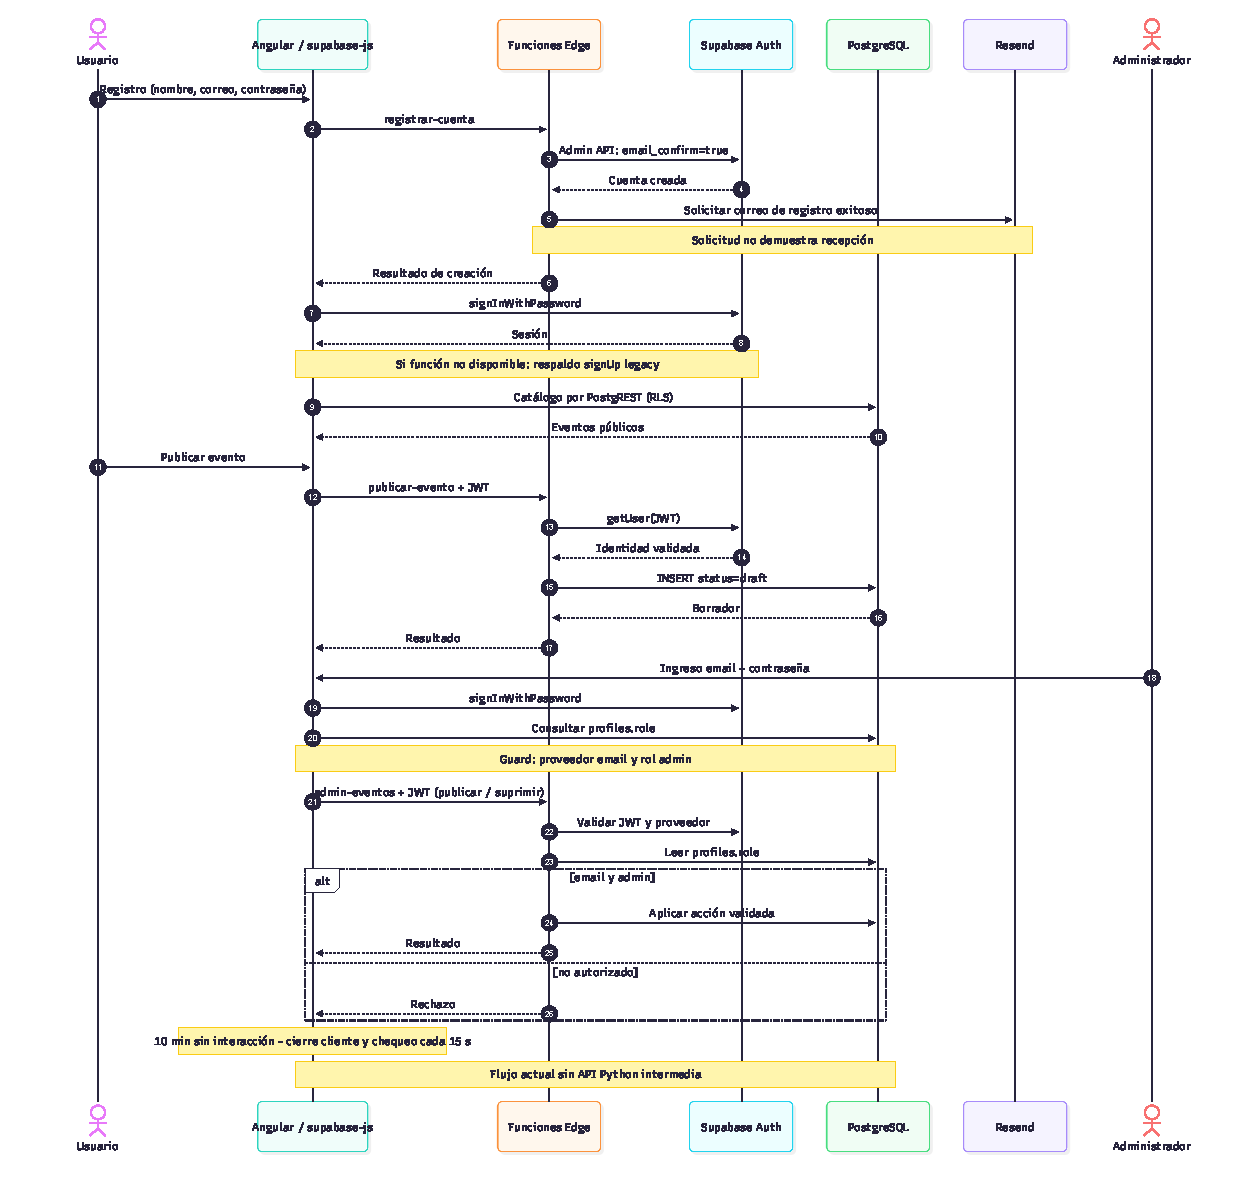
\includegraphics[width=\textwidth]{04_secuencia.pdf}
\caption{Secuencia de registro, sesión, publicación y moderación (editable: Diagramas/04\_secuencia.mmd).}
\label{fig:seq}
\end{figure}

El flujo principal del sistema es la obtención y publicación de eventos: GitHub Actions
ejecuta el pipeline; este restaura el checkpoint, consulta las fuentes con caché
condicional, sanea y deduplica, decide mediante hash qué eventos pasan por IA (con límite
de 40 RPM), reutiliza resultados previos y sincroniza Supabase con upserts idempotentes,
registrando la corrida en \texttt{scrape\_runs}.

\subsection{Componentes y clases}

El diagrama de componentes (Figura~\ref{fig:comp}) muestra los módulos del frontend y del
scraper y su comunicación con la base de datos. En el frontend destacan además el mapa
interactivo real (Leaflet sobre tiles de OpenStreetMap, con pines ligados al catálogo,
popups y geolocalización opcional del usuario) y la página de regreso OAuth
(/auth/callback) integrada en el router. El diagrama de clases (conceptual) refleja
los roles reales del núcleo del scraper verificados en el entregable de Fase 2:
\texttt{EventPipeline}, \texttt{ConnectorFactory}, \texttt{Connector} (Strategy),
\texttt{Event}, \texttt{EventSanitizer}, \texttt{LocationNormalizer},
\texttt{NvidiaService}, \texttt{SupabaseExporter}, \texttt{DatasetExporter} y
\texttt{PipelineState}.

\begin{figure}[H]
\centering
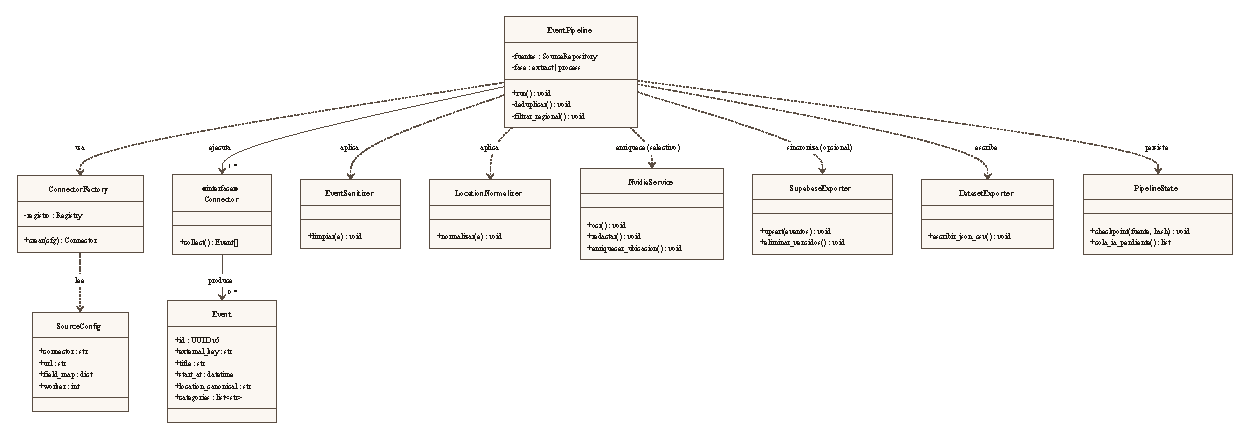
\includegraphics[width=0.95\textwidth]{05_clases.pdf}
\caption{Diagrama de clases conceptual del núcleo del scraper (editable: \texttt{Diagramas/05\_clases.mmd}, Mermaid).}
\label{fig:cls}
\end{figure}

\subsection{Pendientes de UML}

\begin{itemize}[leftmargin=1.4em]
    \item \textbf{Actualizado (31-10-2026):} los diagramas 01, 02 y 04 se ajustan a Supabase directo y funciones Edge; la API intermedia Python no pertenece al flujo actual.
    \item Si el docente exige notación UML estricta: los diagramas de clases
    (05) y casos de uso (03) son versiones conceptuales en Mermaid; una regeneración
    formal añadiría atributos y multiplicidades por clase, y relaciones
    \texttt{<<include>>}/\texttt{<<extend>>} con actores delimitados. La fuente editable
    (\texttt{Diagramas/*.mmd}) es el punto de partida.
    \item Diagrama de clases del frontend (opcional): complementar el (05) con los
    servicios Angular (\texttt{EventosService}, \texttt{ApiService},
    \texttt{RecomendacionService}, \texttt{ViewPreferencesService}).
    \seccionpendiente{confirmar la exigencia del docente, definición de
    responsable y fecha.}
\end{itemize}

% Revisión de Fase 3, 31-10-2026.
\section{Requisitos no funcionales}
\label{sec:rnf}
Se conserva la identificación RNF de la matriz MoSCoW. Implementación no equivale
a cumplimiento medido: los estados siguientes se basan en código local y evidencia
histórica identificada, no en una auditoría actual de producción.
\begin{longtable}{p{1.6cm}p{2.1cm}p{10.5cm}}
\toprule ID & Estado & Fundamento y brecha \\\midrule\endhead
RNF-01 & Parcial & Interfaz de descubrimiento y cuenta implementada. Revalidar defectos de usabilidad del ciclo 11-10-2026. \\
RNF-02 & Parcial & Navegación adaptativa y proyecto Capacitor con APK debug existente. Faltan pruebas nativas en dispositivo y regresión responsive. \\
RNF-03 & Sin medición actual & El tiempo HTTP histórico no mide renderizado ni Core Web Vitals. Faltan volumen, concurrencia y métricas de interacción. \\
RNF-04 & Parcial & Auth, funciones Edge, RLS y secretos de servidor. Registro principal sin verificación de propiedad del buzón; revisar abuso y exposición de datos. La presencia de políticas no acredita su eficacia remota. \\
RNF-05 & Parcial & Guard y servidor exigen profiles.role=admin y proveedor email; visitor/editor/OAuth quedan fuera. Timeout de 10 min en cliente. Faltan pruebas negativas y de revocación. \\
RNF-06 & Parcial & Vercel y evidencia histórica de CI. No se aporta medición de disponibilidad actual ni SLA; el scheduler puede retrasarse. \\
RNF-07 & Diseño implementado & Paginación y upsert en componentes documentados. No se acredita capacidad bajo carga sin medición. \\
RNF-08 & Parcial & Pipeline de saneamiento y deduplicación documentado; revisar muestra actual del catálogo y ubicaciones aproximadas. \\
RNF-09 & Parcial & Servicios, pruebas Vitest, fuentes de diagramas y documentación versionable. Completar ejecución actual y trazabilidad de entrega. \\
RNF-10 & Disponible & Contenido en español y regiones/comunas chilenas; revisión editorial final pendiente. \\
RNF-11 & Parcial & Build web, configuración Vercel y Capacitor presentes; validar reproducción en entorno limpio. Docker no adoptado. \\
RNF-12 & Parcial & Roles ARIA, foco y movimiento reducido en formularios. No se declara conformidad WCAG 2.2 completa sin auditoría y recorrido manual. \\
\bottomrule
\caption{Estado de los RNF al corte documental.}\label{tab:rnfestado}
\end{longtable}

\subsection{Seguridad y limitaciones}
La autenticación comprueba identidad; la autorización administrativa se decide con
\texttt{profiles.role} y se repite en \texttt{admin-eventos}. Ocultar una ruta no
la protege. La clave pública del navegador no es un secreto y exige políticas RLS
correctas; \texttt{service\_role} no debe incorporarse al frontend, capturas ni Git.
El registro sin verificación de correo es una decisión funcional: confirmar mediante
Admin API no acredita que la persona controle el buzón. El correo de bienvenida no
reemplaza esa comprobación. El cierre por inactividad es cliente y puede reiniciarse
con recarga; no se describe como revocación de servidor.

Las notificaciones por correo tienen código en funciones, pero requieren configuración,
recepción comprobada y, para recomendaciones periódicas, invocación programada verificable.
La moderación de eventos está implementada; los reportes ciudadanos y la administración
de organizadores no se dan por completos por existir tablas o rutas. La ocultación
local de fuentes no cambia la ejecución del scraper. La estadística del dashboard es
un cálculo del catálogo, no analítica comercial.

\section{Pruebas y evidencia}
\label{sec:pruebas}
\subsection{Resultados históricos conservados}
El ciclo QA de Vercel del 11-10-2026 registra 13 escenarios: 6 aprobados,
6 con observaciones y 1 fallido, con 13 defectos abiertos. Se conserva en
\texttt{Evidencias\_QA\_Frontend\_2026-10-11} y en la matriz metodológica.
No se cierran defectos sin una nueva ejecución.
La evidencia de CI del scraper conserva cinco ejecuciones trazadas y el run 25
funcional con dos artefactos; su inicio fuera de ventana se registró como DEF-CI-001.
El inventario histórico describe 14 módulos de pruebas del scraper; no se certifica
que ese conteo represente la rama actual.

El anexo previo registra \texttt{ng test --watch=false} con 23/23 el 27-10-2026
y builds anteriores. Son antecedentes, no resultados reproducidos en esta revisión
documental. Los archivos actuales incluyen pruebas de recomendaciones, Supabase y
acciones de interés. No se infiere cobertura de seguridad a partir de su existencia.

\subsection{Plan incremental de cierre}
El Plan de pruebas metodológico incorpora casos F3-01 a F3-10 con resultados
\textbf{pendientes}. Incluyen registro/bienvenida, recuperación, perfil, roles,
OAuth, inactividad, moderación, persistencia, Android y regresión.
Los comandos previstos son \texttt{npm test -- --watch=false},
\texttt{npm run build} y las pruebas focalizadas de cada integración.
Una ejecución debe identificar versión, entorno, responsable y resultado real;
la compilación de esta documentación únicamente acredita generación de entregables.

\section{Despliegue sin Docker}
\label{sec:docker}
La estrategia adoptada no utiliza Docker: el scraper se ejecuta mediante GitHub
Actions, la SPA en Vercel y Android con Capacitor. Supabase es un servicio administrado.
No se agrega un despliegue alternativo ni se declara Docker como implementado.
Su adopción futura requeriría una decisión explícita de arquitectura y pruebas propias.
El Manual técnico describe la reproducción del build y las dependencias de servidor.

\section{Innovación y alcance del MVP}
\label{sec:innovacion}
El valor del proyecto es reunir fuentes culturales heterogéneas y conservar procedencia,
normalización, deduplicación y vigencia en un catálogo consultable. El uso selectivo de
NVIDIA NIM para OCR y enriquecimiento evita repetir trabajo sin cambios; los checkpoints
permiten reanudar procesos. Las recomendaciones al ciudadano se basan en afinidad y
señales explícitas; no se presentan como inferencia de un LLM.

El prototipo académico depende de servicios externos y cuotas configuradas; no dispone
de una infraestructura propia de inferencia. No se afirman ahorros, mejoras de latencia,
usuarios activos ni cifras de eventos actuales sin medición fechada.
El mapa diferencia coordenadas conocidas y ubicaciones aproximadas; esas aproximaciones
no deben presentarse como direcciones exactas.

\subsection{Sostenibilidad: propuesta futura}
El MVP es gratuito y no implementa pagos, suscripciones, venta de datos personales ni
comisiones por entradas. Un eventual contenido patrocinado exigiría validación legal,
comercial y ética, identificación visible, separación de recomendaciones orgánicas y
compatibilidad con las condiciones del hosting. No se certifican condiciones comerciales
vigentes de un proveedor mediante este documento. Cualquier monetización queda fuera
del alcance del cierre actual.


% ---------------------------------------------------------- ESTÁNDARES Y EVIDENCIA
\section{Estándares de desarrollo y evidencia del avance}
\label{sec:estandares}

Esta sección declara los estándares de la industria bajo los que se desarrolla el
proyecto, cómo se organiza la evidencia del avance bajo control de versiones y
dónde pueden verificarse los aportes por integrante; responde así a los criterios
de evaluación de "evidencias que cumplan estándares de desarrollo",
"estructura y nombres" y "aporte por integrante".

\subsection{Estándares y prácticas de la industria aplicados}

\begin{table}[ht]
\centering\small
\renewcommand{\arraystretch}{1.3}
\begin{tabular}{p{4.6cm} p{4.2cm} p{5.0cm}}
\toprule
\textbf{Estándar / práctica} & \textbf{Dónde se aplica} & \textbf{Evidencia verificable} \\
\midrule
Patrones orientados a WCAG 2.2 en las interfaces (avisos semánticos, foco visible,
objetivos táctiles, movimiento reducido) &
Login, recuperación de contraseña y publicación de eventos &
\texttt{role="alert"} y \texttt{role="status"} con botón de cierre y tokens de color;
Novedades de Fase 3, sección 6. \\
OAuth 2.0 y PKCE (RFC 6749, RFC 7636) en el regreso de proveedores externos &
\texttt{/auth/callback} (Angular Router) &
\texttt{auth-callback.page.ts} y flujo \texttt{signInWithOAuth} de supabase-js. \\
Control de acceso en la base de datos por mínimo
privilegio (RLS de PostgreSQL) &
Modelo documentado de catálogo y perfil; validar políticas remotas &
Migraciones SQL (repositorio oficial del scraper) y vista \texttt{public\_event\_catalog}. \\
Sincronización idempotente por upsert y conciliación configurable &
\texttt{SupabaseExporter} del scraper &
Pipeline por lotes configurable y pruebas \texttt{test\_supabase.py}. \\
Integración continua con compuerta de calidad (las pruebas bloquean la publicación de datos) &
Workflow \texttt{scrape-events.yml} &
Run \#12: falla de pruebas impide extracción/sincronización; runs \#25 en verde. \\
Separación de secretos por entorno (configuración 12-factor, sin claves en el cliente) &
Backend y despliegues &
\texttt{.env.example} en todos los entregables, GitHub Secrets y Edge Functions
\texttt{admin-account} y funciones de recuperación con clave \texttt{service\_role} solo en Supabase. \\
Patrones de arquitectura de software (Strategy, Factory, Repository, Adapter,
Chain of Responsibility, Bulkhead, Cache-Aside) &
Scraper y frontend Angular &
Documentación interna de ambos entregables y pruebas con inyección de
dependencias; servicios Angular con inyección estándar. \\
Convenciones de estilo y verificación automática de dependencias &
Repositorios del proyecto &
Python snake\_case con \texttt{requirements.txt}; Angular 22 standalone con
\texttt{angular-eslint} y \texttt{package-lock.json}; SCSS por token de diseño
(\texttt{\_tokens.scss}). \\
Responsividad y app instalable &
Frontend web y Android &
Navegación dual móvil/escritorio de Ionic, \texttt{manifest.webmanifest} y el build
APK de Capacitor (Novedades de Fase 3, sección 4). \\
\bottomrule
\end{tabular}
\caption{Estándares de desarrollo industriales adoptados con su evidencia en el repositorio.}
\label{tab:estandares}
\end{table}

\subsection{Estructura de evidencias, nomenclatura y control de versiones}

La carpeta raíz del proyecto se organiza por fase según la estructura oficial del
curso (``Resumen evidencias.xlsx''): \texttt{Fase 1/2/3}, cada una con sus
\texttt{Evidencias Individuales/}, \texttt{Evidencias Grupales/} y
\texttt{Evidencias Proyecto/} según aplique. La nomenclatura es uniforme: nombres
descriptivos en español, fechas en formato dd-mm-aaaa y estados explícitos
(\emph{Pendiente de completar por el equipo}, parciales e implementados).

El control de versiones es el respaldo central del avance: la bitácora
\nolinkurl{REGISTRO_CAMBIOS_DOCUMENTACION.md} registra fecha, origen, acciones, verificación y
archivos de cada ciclo documental (secciones 1--28); los commits del repositorio
oficial del scraper muestran la línea de tiempo del backend (antecedente histórico: corrección del reloj de pruebas, commit \texttt{d201b0a}). La entrega debe excluir auxiliares LaTeX, dependencias y secretos, pero incluir los PDFs y fuentes evaluables. Esta revisión no certifica qué archivos están guardados en Git; el equipo debe registrar el commit y comprobar su contenido antes de entregar.

\subsection{Roles planificados y trazabilidad individual pendiente}

\begin{table}[ht]
\centering\small
\renewcommand{\arraystretch}{1.3}
\begin{tabular}{p{4.0cm} p{9.6cm}}
\toprule
\textbf{Integrante} & \textbf{Área de responsabilidad según planificación} \\
\midrule
Roberto Riffo (líder) &
Frontend Angular/Ionic (páginas, layouts y design system), gestión del proyecto
y documento de metodología. \\
José Miguel Moncada &
Base de datos, plan de pruebas y ejecución QA (ciclo del 11-10-2026 con 13
escenarios y matriz de defectos); recomendaciones e informe QA de Fase 3.
\\
David Herrera &
Backend e integraciones: scraper, su CI \texttt{scrape-events.yml}, migraciones SQL y
Edge Functions \texttt{admin-account} / \texttt{reset-password}. \\
\bottomrule
\end{tabular}
\caption{Distribución planificada según el design brief; no certifica autoría de cambios. Adjuntar commits o actas reales para demostrar aportes.}
\label{tab:aportes}
\end{table}

% ---------------------------------------------------------- CIERRE
\section{Trazabilidad documental}
\label{sec:traza}

Cada afirmación de este documento proviene de las siguientes fuentes verificables:

\begin{table}[h]
\centering\small
\renewcommand{\arraystretch}{1.25}
\begin{tabular}{p{5.2cm} p{8.6cm}}
\toprule
\textbf{Sección} & \textbf{Evidencia utilizada} \\
\midrule
Arquitectura general, scraper y frontend &
Entregables del scraper y frontend incluidos como evidencias de sistema en Fase 2;
\texttt{package.json}, \texttt{app.routes.ts}, \texttt{supabase.service.ts},
\texttt{api.service.ts}, Edge Functions y diagramas técnicos de Fase 2.
Integración frontend--Supabase implementada y verificada en TypeScript
(catálogo real directo, autenticación y OAuth preparado). \\
Modelo de datos &
Documentación de base de datos incluida en el entregable del scraper de Fase 2,
modelo DBML, diccionario de tablas y
\texttt{DB\_evento\_cultural.pdf} (Fase 1). \\
Diagramas UML &
Rutas y servicios reales del frontend; clases y patrones documentados del scraper;
matriz MoSCoW de Fase 1. Los siete diagramas (01--07) comparten estándar visual,
fueron pulidos y reexportados el 27-09-2026 y el ER (06) fue actualizado el 03-10-2026. \\
Requisitos no funcionales &
Matriz MoSCoW de requerimientos (Fase 1) y
evidencia de código por requisito. \\
Pruebas &
Carpeta \texttt{tests/} del scraper (14 módulos, aproximadamente 1.900 líneas),
sección ``Pruebas'' de su README y configuración Vitest del frontend. \\
Docker &
Inspección completa de ambos entregables (sin Dockerfile ni compose) y
\texttt{CONTENIDO\_DEL\_REPOSITORIO.md}. \\
Innovación &
Design brief de Fase 1, matriz MoSCoW, tabla de fuentes del README del scraper y
funcionalidad ``para ti'' del frontend. \\
\bottomrule
\end{tabular}
\caption{Trazabilidad entre secciones del documento y evidencia del repositorio.}
\label{tab:traza}
\end{table}

Los cambios y pendientes vigentes de Fase 3 se resumen en el anexo
\nolinkurl{Novedades_desde_Fase2.md} de \texttt{Fase 3/Evidencias Grupales/} y en la bitácora
\nolinkurl{REGISTRO_CAMBIOS_DOCUMENTACION.md} de la raíz.

% ---------------------------------------------------------- REFERENCIAS
\section*{Referencias}
\addcontentsline{toc}{section}{Referencias}

Este documento cita los siguientes estándares y fuentes primarias (formato,
estándar/autor, nombre, versión o RFC y URL de consulta):

\begin{enumerate}[leftmargin=1.6em, label=\textsuperscript{[\arabic*]}]
    \item World Wide Web Consortium. \emph{Web Content Accessibility Guidelines (WCAG) 2.2}. W3C
    Recommendation, oct. 2023. \url{https://www.w3.org/TR/WCAG22/}.
    \item Hardt, D. (ed.). \emph{The OAuth 2.0 Authorization Framework}. RFC 6749, IETF, 2012.
    \url{https://www.rfc-editor.org/rfc/rfc6749}.
    \item Sakimura, N., Bradley, J. y Jones, M. \emph{Proof Key for Code Exchange} (PKCE).
    RFC 7636, IETF, 2015. \url{https://www.rfc-editor.org/rfc/rfc7636}.
    \item PostgreSQL Global Development Group. \emph{PostgreSQL Documentation: Row Security
    Policies}. \url{https://www.postgresql.org/docs/current/ddl-rowsecurity.html}.
    \item OpenStreetMap Foundation. \emph{Nominatim Usage Policy} (geocodificación de respaldo
    del mapa). \url{https://operations.osmfoundation.org/policies/nominatim/}.
    \item Proyecto Mermaid. \emph{Mermaid: documentación oficial} (herramienta utilizada para los diagramas propios 01--07). \url{https://mermaid.js.org/intro/}.
    \item Google LLC (equipo Angular). \emph{Angular Style Guide} y documentación de
    componentes standalone (v20--22). \url{https://angular.dev/style-guide}.
    \item Ionic. \emph{Ionic Framework documentation} (v9) para navegación responsiva
    móvil/escritorio. \url{https://ionicframework.com/docs}.
    \item Supabase. \emph{Supabase documentation} (Row Level Security, Edge Functions y
    Inicio de sesión con GoTrue). \url{https://supabase.com/docs}.
    \item NVIDIA Corporation. \emph{NVIDIA NIM for microservices} (API de inferencia de OCR y
    redacción). \url{https://www.nvidia.com/en-us/ai-data-science/products/nim-microservices/}.
\end{enumerate}

\end{document}
